\documentclass[12pt]{article}
\usepackage{graphicx}

\title{ASTR 605: ISM}
\author{Laurel Farris}
\date{23 September 2015}

% Increase margins (manually)
  % Sides (odd- and even-numbered pages)
    \addtolength{\oddsidemargin}{-0.875in}
    \addtolength{\evensidemargin}{-0.875in}
    \addtolength{\textwidth}{1.75in}
  % Top/bottom
    \addtolength{\topmargin}{-0.875in}
    \addtolength{\textheight}{1.75in}

\begin{document}    % Put \end{document} last line of doc.

\maketitle


\section{Question 3}
\subsection{Part (a)}

% Insert figure

\begin{figure}[h]   % h - 'here' as in put the figure where I tell you to.
\centering
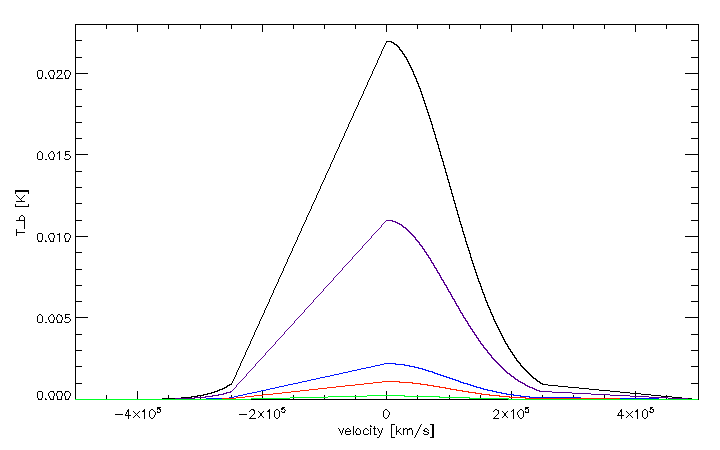
\includegraphics[width=5.0in]{plot_a.png}
\caption{This plot shows the thermally broadened 
 HI line profile sampled at channel widths of 
0.5 km/s. The brightness temperature is plotted as a function of velocity, 
and serves as a representation of the intensity. Each of the five
 profiles represents a different column density, in units of 
$10^{21}$ cm$^{-3}$. From the top down: N=0.1 (black), N=0.5 (purple), 
N=1.0 (blue), N=5.0 (red), and N=10 (green). }
\label{plot_a}
\end{figure}


\newpage  % Jump to a new page after previous section
\subsection{Part (b)}
\begin{figure}[h]   % h - 'here' as in put the figure where I tell you to.
\centering
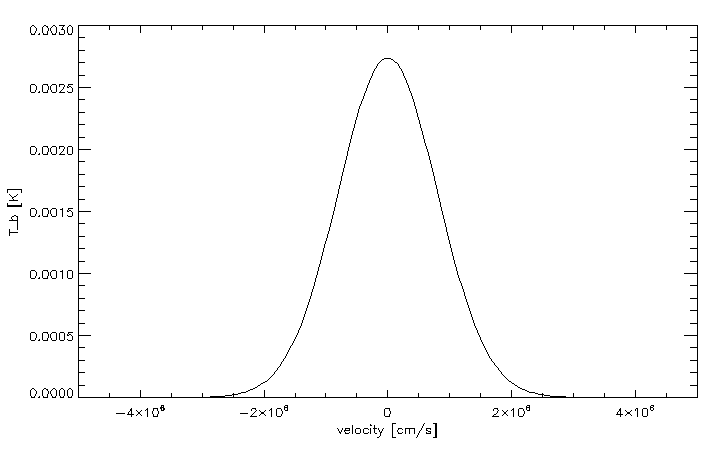
\includegraphics[width=5.0in]{partb.png}
\caption{This plot shows a single H1 line profile at a column density
of N = 10$^{21}$ cm$^{-3}$}
\label{plot_b}
\end{figure}

\end{document}
%----------------------------------------------------------------------------%


% write out a fraction
%$\frac{1}{4}$   % to print 1/4 as a nice fraction
% Put dollar signs around any symbol, e.g. $L$ to put it in equation,
%  or italic form within text (don't have to make equation).


% Equations
%\begin{equation}
%  something...
%\end{equation}



